\subsection{Client Interface}
\label{sec:client_interface}

After login, the \aclient[] is greeted with the \textit{main} screen, wich gives three posebilities:
\begin{itemize}
	\item Add problem
	\item My problems
	\item Search for problem(s)
\end{itemize}

\paragraph{Add problem} as the name dictates, initiates the process of adding a specific problem to the system. Process starts by selecting what kind of problem the \aclient[] has. This is done by selecting \textit{tags} which describes the problem. Tags are grouped under categories. Each tag can only exist under one category, however if the need arises, it is possible to create a duplicate tag under another category. The problem is ``categorized'' when it has tags associated with it.
When the \aclient[] is satisfied with the categorization of his/hers problem, he/she can click ``Search'', which will make the system search for problems with similair categorization
\paragraph{My problems}
\paragraph{Search for problem(s)}



\begin{figure}[h]
\begin{center}
 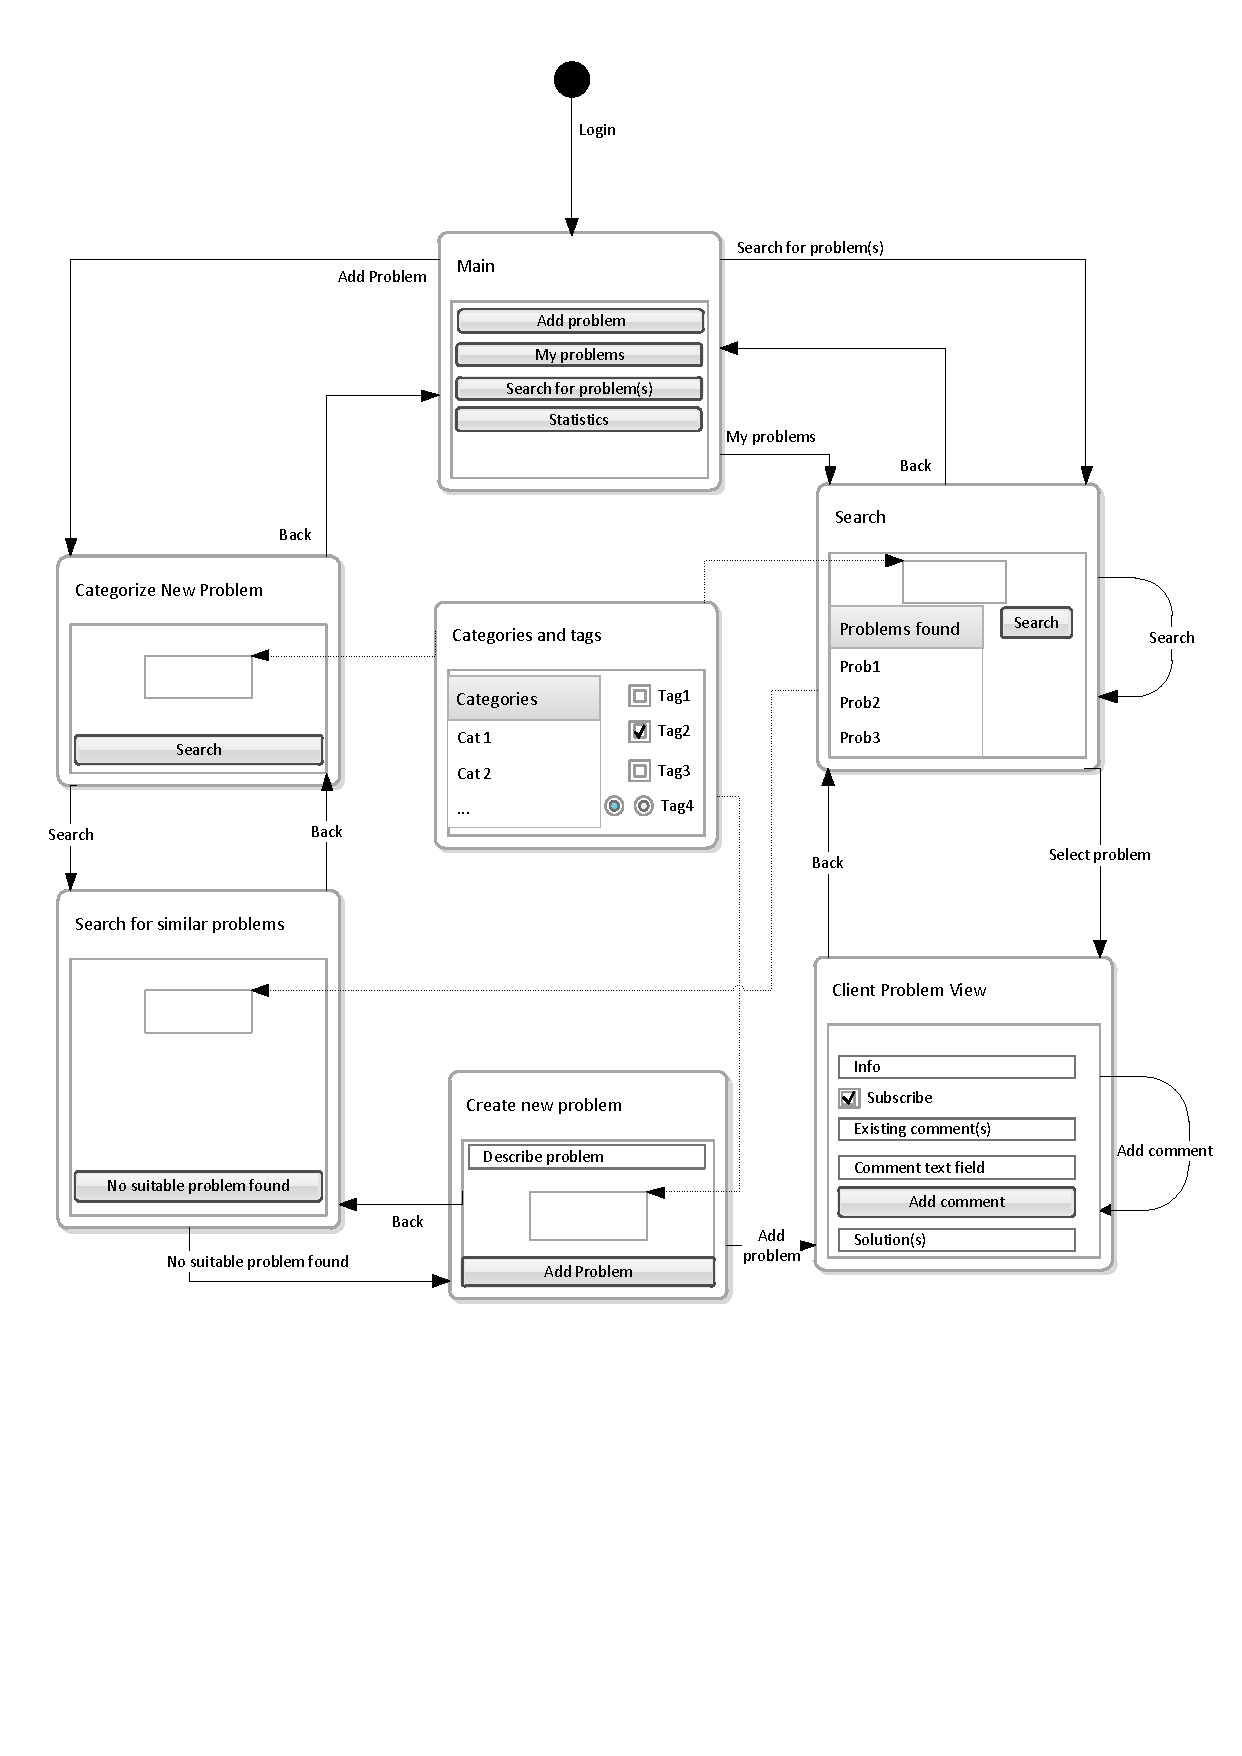
\includegraphics[scale=0.70]{input/application_domain_analysis/client_interface}
\caption{\Client[] interface}
\label{fig:client_interface}
\end{center}
\end{figure}

